% Created by tikzDevice version 0.9 on 2016-01-12 22:38:49
% !TEX encoding = UTF-8 Unicode
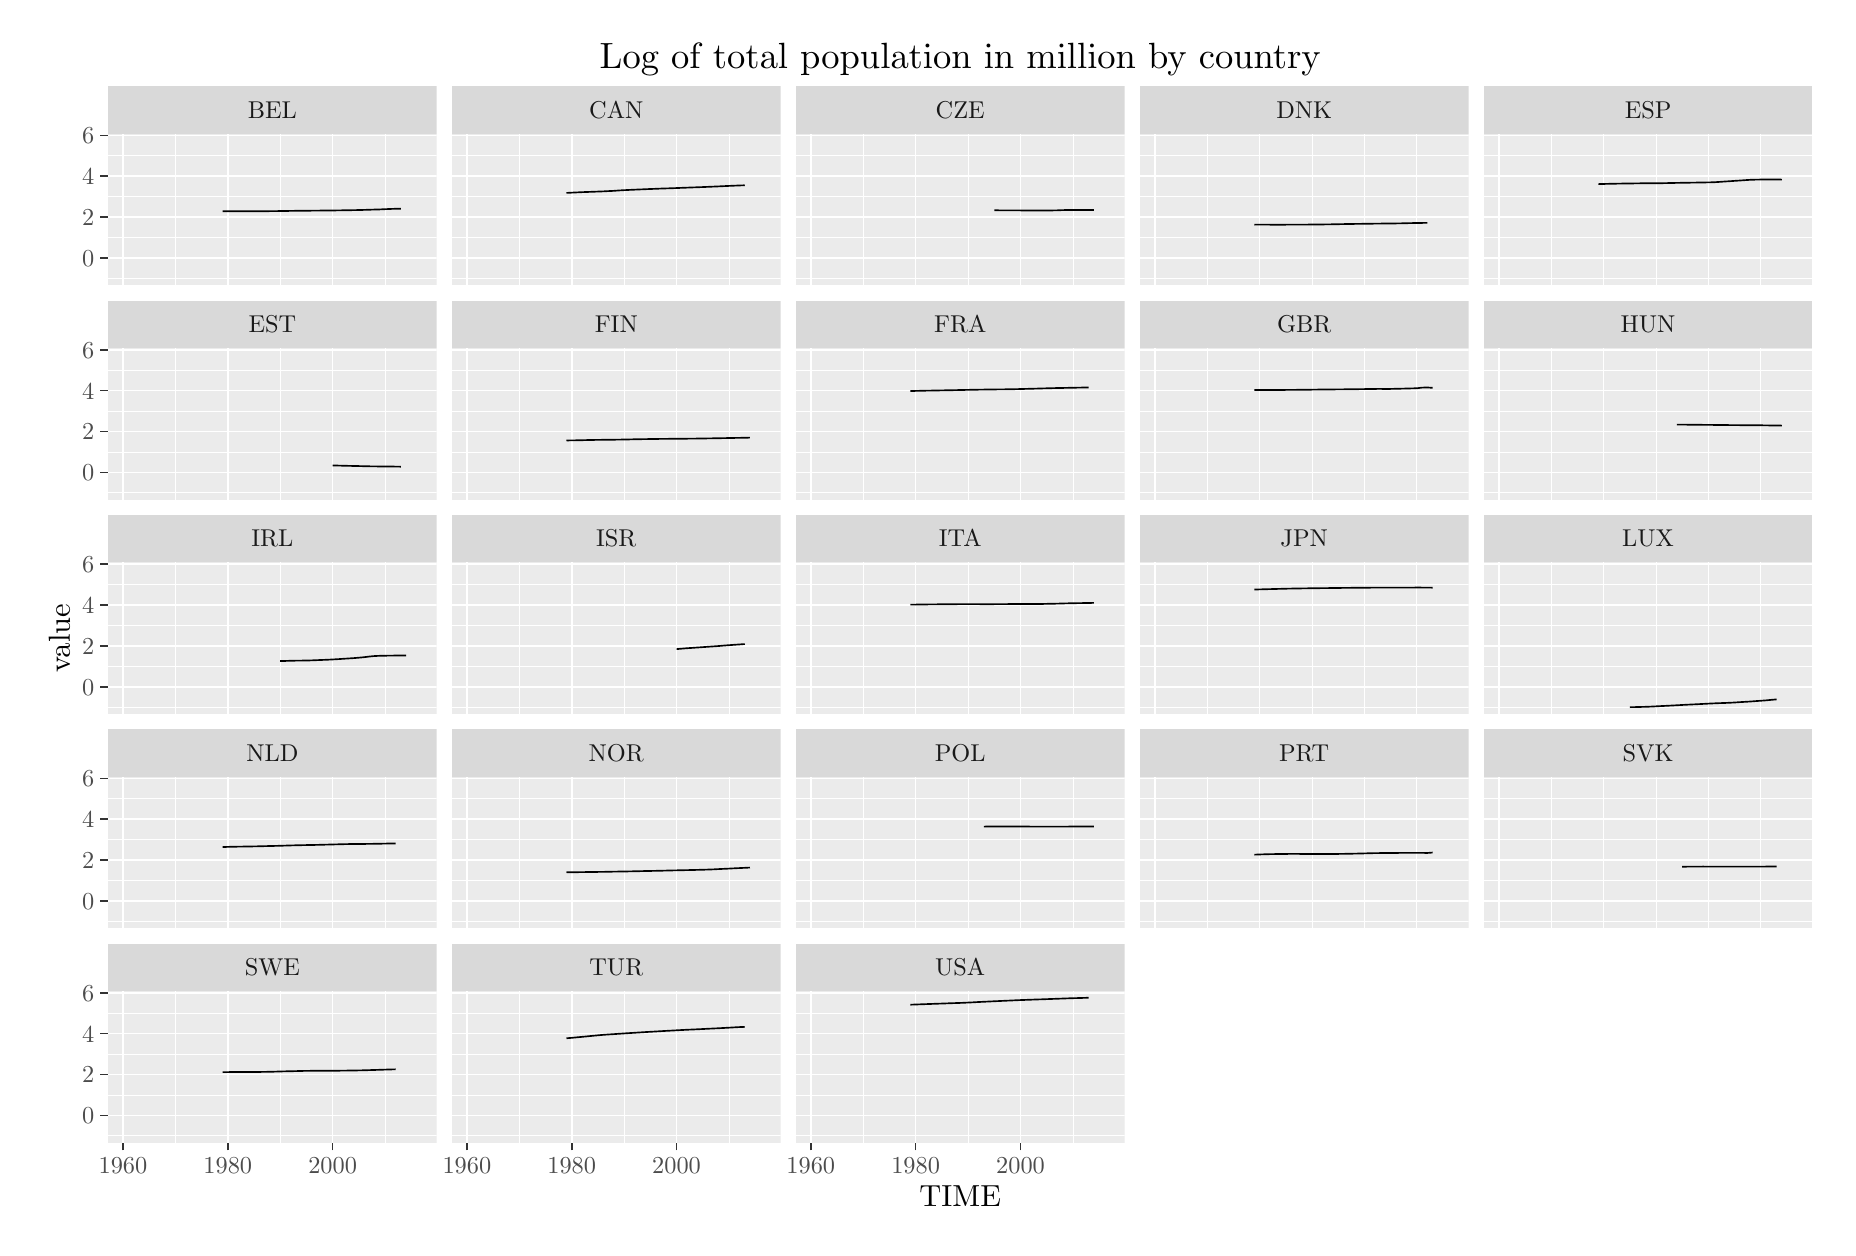
\begin{tikzpicture}[x=1pt,y=1pt]
\definecolor{fillColor}{RGB}{255,255,255}
\path[use as bounding box,fill=fillColor,fill opacity=0.00] (0,0) rectangle (650.43,433.62);
\begin{scope}
\path[clip] (  0.00,  0.00) rectangle (650.43,433.62);
\definecolor{drawColor}{RGB}{255,255,255}
\definecolor{fillColor}{RGB}{255,255,255}

\path[draw=drawColor,line width= 0.6pt,line join=round,line cap=round,fill=fillColor] (  0.00,  0.00) rectangle (650.43,433.62);
\end{scope}
\begin{scope}
\path[clip] ( 29.02,340.48) rectangle (147.81,395.37);
\definecolor{fillColor}{gray}{0.92}

\path[fill=fillColor] ( 29.02,340.48) rectangle (147.81,395.37);
\definecolor{drawColor}{RGB}{255,255,255}

\path[draw=drawColor,line width= 0.3pt,line join=round] ( 29.02,343.00) --
	(147.81,343.00);

\path[draw=drawColor,line width= 0.3pt,line join=round] ( 29.02,357.76) --
	(147.81,357.76);

\path[draw=drawColor,line width= 0.3pt,line join=round] ( 29.02,372.53) --
	(147.81,372.53);

\path[draw=drawColor,line width= 0.3pt,line join=round] ( 29.02,387.29) --
	(147.81,387.29);

\path[draw=drawColor,line width= 0.3pt,line join=round] ( 53.37,340.48) --
	( 53.37,395.37);

\path[draw=drawColor,line width= 0.3pt,line join=round] ( 91.26,340.48) --
	( 91.26,395.37);

\path[draw=drawColor,line width= 0.3pt,line join=round] (129.15,340.48) --
	(129.15,395.37);

\path[draw=drawColor,line width= 0.6pt,line join=round] ( 29.02,350.38) --
	(147.81,350.38);

\path[draw=drawColor,line width= 0.6pt,line join=round] ( 29.02,365.15) --
	(147.81,365.15);

\path[draw=drawColor,line width= 0.6pt,line join=round] ( 29.02,379.91) --
	(147.81,379.91);

\path[draw=drawColor,line width= 0.6pt,line join=round] ( 29.02,394.67) --
	(147.81,394.67);

\path[draw=drawColor,line width= 0.6pt,line join=round] ( 34.42,340.48) --
	( 34.42,395.37);

\path[draw=drawColor,line width= 0.6pt,line join=round] ( 72.31,340.48) --
	( 72.31,395.37);

\path[draw=drawColor,line width= 0.6pt,line join=round] (110.20,340.48) --
	(110.20,395.37);
\definecolor{drawColor}{RGB}{0,0,0}

\path[draw=drawColor,line width= 0.6pt,line join=round] ( 70.42,367.27) --
	( 72.31,367.27) --
	( 74.21,367.27) --
	( 76.10,367.27) --
	( 78.00,367.27) --
	( 79.89,367.27) --
	( 81.78,367.27) --
	( 83.68,367.28) --
	( 85.57,367.28) --
	( 87.47,367.31) --
	( 89.36,367.33) --
	( 91.26,367.35) --
	( 93.15,367.38) --
	( 95.05,367.41) --
	( 96.94,367.44) --
	( 98.83,367.46) --
	(100.73,367.48) --
	(102.62,367.49) --
	(104.52,367.51) --
	(106.41,367.53) --
	(108.31,367.54) --
	(110.20,367.56) --
	(112.10,367.59) --
	(113.99,367.62) --
	(115.88,367.65) --
	(117.78,367.68) --
	(119.67,367.72) --
	(121.57,367.77) --
	(123.46,367.83) --
	(125.36,367.89) --
	(127.25,367.94) --
	(129.15,368.03) --
	(131.04,368.11) --
	(132.93,368.17) --
	(134.83,368.20);
\end{scope}
\begin{scope}
\path[clip] (153.31,340.48) rectangle (272.09,395.37);
\definecolor{fillColor}{gray}{0.92}

\path[fill=fillColor] (153.31,340.48) rectangle (272.09,395.37);
\definecolor{drawColor}{RGB}{255,255,255}

\path[draw=drawColor,line width= 0.3pt,line join=round] (153.31,343.00) --
	(272.09,343.00);

\path[draw=drawColor,line width= 0.3pt,line join=round] (153.31,357.76) --
	(272.09,357.76);

\path[draw=drawColor,line width= 0.3pt,line join=round] (153.31,372.53) --
	(272.09,372.53);

\path[draw=drawColor,line width= 0.3pt,line join=round] (153.31,387.29) --
	(272.09,387.29);

\path[draw=drawColor,line width= 0.3pt,line join=round] (177.65,340.48) --
	(177.65,395.37);

\path[draw=drawColor,line width= 0.3pt,line join=round] (215.54,340.48) --
	(215.54,395.37);

\path[draw=drawColor,line width= 0.3pt,line join=round] (253.43,340.48) --
	(253.43,395.37);

\path[draw=drawColor,line width= 0.6pt,line join=round] (153.31,350.38) --
	(272.09,350.38);

\path[draw=drawColor,line width= 0.6pt,line join=round] (153.31,365.15) --
	(272.09,365.15);

\path[draw=drawColor,line width= 0.6pt,line join=round] (153.31,379.91) --
	(272.09,379.91);

\path[draw=drawColor,line width= 0.6pt,line join=round] (153.31,394.67) --
	(272.09,394.67);

\path[draw=drawColor,line width= 0.6pt,line join=round] (158.71,340.48) --
	(158.71,395.37);

\path[draw=drawColor,line width= 0.6pt,line join=round] (196.59,340.48) --
	(196.59,395.37);

\path[draw=drawColor,line width= 0.6pt,line join=round] (234.48,340.48) --
	(234.48,395.37);
\definecolor{drawColor}{RGB}{0,0,0}

\path[draw=drawColor,line width= 0.6pt,line join=round] (194.70,373.90) --
	(196.59,374.00) --
	(198.49,374.09) --
	(200.38,374.18) --
	(202.28,374.25) --
	(204.17,374.32) --
	(206.07,374.39) --
	(207.96,374.46) --
	(209.85,374.56) --
	(211.75,374.65) --
	(213.64,374.79) --
	(215.54,374.90) --
	(217.43,374.99) --
	(219.33,375.08) --
	(221.22,375.16) --
	(223.12,375.24) --
	(225.01,375.32) --
	(226.90,375.39) --
	(228.80,375.47) --
	(230.69,375.53) --
	(232.59,375.59) --
	(234.48,375.66) --
	(236.38,375.74) --
	(238.27,375.81) --
	(240.17,375.88) --
	(242.06,375.95) --
	(243.95,376.02) --
	(245.85,376.10) --
	(247.74,376.18) --
	(249.64,376.26) --
	(251.53,376.35) --
	(253.43,376.44) --
	(255.32,376.52) --
	(257.22,376.60) --
	(259.11,376.66);
\end{scope}
\begin{scope}
\path[clip] (277.59,340.48) rectangle (396.37,395.37);
\definecolor{fillColor}{gray}{0.92}

\path[fill=fillColor] (277.59,340.48) rectangle (396.37,395.37);
\definecolor{drawColor}{RGB}{255,255,255}

\path[draw=drawColor,line width= 0.3pt,line join=round] (277.59,343.00) --
	(396.37,343.00);

\path[draw=drawColor,line width= 0.3pt,line join=round] (277.59,357.76) --
	(396.37,357.76);

\path[draw=drawColor,line width= 0.3pt,line join=round] (277.59,372.53) --
	(396.37,372.53);

\path[draw=drawColor,line width= 0.3pt,line join=round] (277.59,387.29) --
	(396.37,387.29);

\path[draw=drawColor,line width= 0.3pt,line join=round] (301.93,340.48) --
	(301.93,395.37);

\path[draw=drawColor,line width= 0.3pt,line join=round] (339.82,340.48) --
	(339.82,395.37);

\path[draw=drawColor,line width= 0.3pt,line join=round] (377.71,340.48) --
	(377.71,395.37);

\path[draw=drawColor,line width= 0.6pt,line join=round] (277.59,350.38) --
	(396.37,350.38);

\path[draw=drawColor,line width= 0.6pt,line join=round] (277.59,365.15) --
	(396.37,365.15);

\path[draw=drawColor,line width= 0.6pt,line join=round] (277.59,379.91) --
	(396.37,379.91);

\path[draw=drawColor,line width= 0.6pt,line join=round] (277.59,394.67) --
	(396.37,394.67);

\path[draw=drawColor,line width= 0.6pt,line join=round] (282.99,340.48) --
	(282.99,395.37);

\path[draw=drawColor,line width= 0.6pt,line join=round] (320.87,340.48) --
	(320.87,395.37);

\path[draw=drawColor,line width= 0.6pt,line join=round] (358.76,340.48) --
	(358.76,395.37);
\definecolor{drawColor}{RGB}{0,0,0}

\path[draw=drawColor,line width= 0.6pt,line join=round] (349.29,367.62) --
	(351.19,367.61) --
	(353.08,367.60) --
	(354.97,367.59) --
	(356.87,367.58) --
	(358.76,367.58) --
	(360.66,367.54) --
	(362.55,367.53) --
	(364.45,367.53) --
	(366.34,367.53) --
	(368.24,367.55) --
	(370.13,367.57) --
	(372.02,367.61) --
	(373.92,367.69) --
	(375.81,367.73) --
	(377.71,367.75) --
	(379.60,367.74) --
	(381.50,367.75) --
	(383.39,367.75) --
	(385.29,367.76);
\end{scope}
\begin{scope}
\path[clip] (401.87,340.48) rectangle (520.65,395.37);
\definecolor{fillColor}{gray}{0.92}

\path[fill=fillColor] (401.87,340.48) rectangle (520.65,395.37);
\definecolor{drawColor}{RGB}{255,255,255}

\path[draw=drawColor,line width= 0.3pt,line join=round] (401.87,343.00) --
	(520.65,343.00);

\path[draw=drawColor,line width= 0.3pt,line join=round] (401.87,357.76) --
	(520.65,357.76);

\path[draw=drawColor,line width= 0.3pt,line join=round] (401.87,372.53) --
	(520.65,372.53);

\path[draw=drawColor,line width= 0.3pt,line join=round] (401.87,387.29) --
	(520.65,387.29);

\path[draw=drawColor,line width= 0.3pt,line join=round] (426.21,340.48) --
	(426.21,395.37);

\path[draw=drawColor,line width= 0.3pt,line join=round] (464.10,340.48) --
	(464.10,395.37);

\path[draw=drawColor,line width= 0.3pt,line join=round] (501.99,340.48) --
	(501.99,395.37);

\path[draw=drawColor,line width= 0.6pt,line join=round] (401.87,350.38) --
	(520.65,350.38);

\path[draw=drawColor,line width= 0.6pt,line join=round] (401.87,365.15) --
	(520.65,365.15);

\path[draw=drawColor,line width= 0.6pt,line join=round] (401.87,379.91) --
	(520.65,379.91);

\path[draw=drawColor,line width= 0.6pt,line join=round] (401.87,394.67) --
	(520.65,394.67);

\path[draw=drawColor,line width= 0.6pt,line join=round] (407.27,340.48) --
	(407.27,395.37);

\path[draw=drawColor,line width= 0.6pt,line join=round] (445.16,340.48) --
	(445.16,395.37);

\path[draw=drawColor,line width= 0.6pt,line join=round] (483.04,340.48) --
	(483.04,395.37);
\definecolor{drawColor}{RGB}{0,0,0}

\path[draw=drawColor,line width= 0.6pt,line join=round] (443.26,362.43) --
	(445.16,362.44) --
	(447.05,362.44) --
	(448.94,362.43) --
	(450.84,362.43) --
	(452.73,362.42) --
	(454.63,362.43) --
	(456.52,362.44) --
	(458.42,362.45) --
	(460.31,362.45) --
	(462.21,362.46) --
	(464.10,362.47) --
	(465.99,362.49) --
	(467.89,362.51) --
	(469.78,362.54) --
	(471.68,362.56) --
	(473.57,362.60) --
	(475.47,362.64) --
	(477.36,362.67) --
	(479.26,362.70) --
	(481.15,362.72) --
	(483.04,362.75) --
	(484.94,362.77) --
	(486.83,362.80) --
	(488.73,362.82) --
	(490.62,362.84) --
	(492.52,362.86) --
	(494.41,362.88) --
	(496.31,362.91) --
	(498.20,362.96) --
	(500.09,363.00) --
	(501.99,363.03) --
	(503.88,363.06) --
	(505.78,363.09);
\end{scope}
\begin{scope}
\path[clip] (526.15,340.48) rectangle (644.93,395.37);
\definecolor{fillColor}{gray}{0.92}

\path[fill=fillColor] (526.15,340.48) rectangle (644.93,395.37);
\definecolor{drawColor}{RGB}{255,255,255}

\path[draw=drawColor,line width= 0.3pt,line join=round] (526.15,343.00) --
	(644.93,343.00);

\path[draw=drawColor,line width= 0.3pt,line join=round] (526.15,357.76) --
	(644.93,357.76);

\path[draw=drawColor,line width= 0.3pt,line join=round] (526.15,372.53) --
	(644.93,372.53);

\path[draw=drawColor,line width= 0.3pt,line join=round] (526.15,387.29) --
	(644.93,387.29);

\path[draw=drawColor,line width= 0.3pt,line join=round] (550.49,340.48) --
	(550.49,395.37);

\path[draw=drawColor,line width= 0.3pt,line join=round] (588.38,340.48) --
	(588.38,395.37);

\path[draw=drawColor,line width= 0.3pt,line join=round] (626.27,340.48) --
	(626.27,395.37);

\path[draw=drawColor,line width= 0.6pt,line join=round] (526.15,350.38) --
	(644.93,350.38);

\path[draw=drawColor,line width= 0.6pt,line join=round] (526.15,365.15) --
	(644.93,365.15);

\path[draw=drawColor,line width= 0.6pt,line join=round] (526.15,379.91) --
	(644.93,379.91);

\path[draw=drawColor,line width= 0.6pt,line join=round] (526.15,394.67) --
	(644.93,394.67);

\path[draw=drawColor,line width= 0.6pt,line join=round] (531.55,340.48) --
	(531.55,395.37);

\path[draw=drawColor,line width= 0.6pt,line join=round] (569.44,340.48) --
	(569.44,395.37);

\path[draw=drawColor,line width= 0.6pt,line join=round] (607.33,340.48) --
	(607.33,395.37);
\definecolor{drawColor}{RGB}{0,0,0}

\path[draw=drawColor,line width= 0.6pt,line join=round] (567.54,377.09) --
	(569.44,377.14) --
	(571.33,377.19) --
	(573.23,377.23) --
	(575.12,377.26) --
	(577.01,377.30) --
	(578.91,377.32) --
	(580.80,377.34) --
	(582.70,377.37) --
	(584.59,377.38) --
	(586.49,377.39) --
	(588.38,377.40) --
	(590.28,377.41) --
	(592.17,377.45) --
	(594.06,377.49) --
	(595.96,377.53) --
	(597.85,377.56) --
	(599.75,377.59) --
	(601.64,377.62) --
	(603.54,377.65) --
	(605.43,377.68) --
	(607.33,377.71) --
	(609.22,377.75) --
	(611.11,377.87) --
	(613.01,378.01) --
	(614.90,378.12) --
	(616.80,378.26) --
	(618.69,378.38) --
	(620.59,378.52) --
	(622.48,378.64) --
	(624.38,378.70) --
	(626.27,378.73) --
	(628.16,378.76) --
	(630.06,378.77) --
	(631.95,378.74) --
	(633.85,378.72);
\end{scope}
\begin{scope}
\path[clip] ( 29.02,263.03) rectangle (147.81,317.92);
\definecolor{fillColor}{gray}{0.92}

\path[fill=fillColor] ( 29.02,263.03) rectangle (147.81,317.92);
\definecolor{drawColor}{RGB}{255,255,255}

\path[draw=drawColor,line width= 0.3pt,line join=round] ( 29.02,265.55) --
	(147.81,265.55);

\path[draw=drawColor,line width= 0.3pt,line join=round] ( 29.02,280.31) --
	(147.81,280.31);

\path[draw=drawColor,line width= 0.3pt,line join=round] ( 29.02,295.08) --
	(147.81,295.08);

\path[draw=drawColor,line width= 0.3pt,line join=round] ( 29.02,309.84) --
	(147.81,309.84);

\path[draw=drawColor,line width= 0.3pt,line join=round] ( 53.37,263.03) --
	( 53.37,317.92);

\path[draw=drawColor,line width= 0.3pt,line join=round] ( 91.26,263.03) --
	( 91.26,317.92);

\path[draw=drawColor,line width= 0.3pt,line join=round] (129.15,263.03) --
	(129.15,317.92);

\path[draw=drawColor,line width= 0.6pt,line join=round] ( 29.02,272.93) --
	(147.81,272.93);

\path[draw=drawColor,line width= 0.6pt,line join=round] ( 29.02,287.70) --
	(147.81,287.70);

\path[draw=drawColor,line width= 0.6pt,line join=round] ( 29.02,302.46) --
	(147.81,302.46);

\path[draw=drawColor,line width= 0.6pt,line join=round] ( 29.02,317.22) --
	(147.81,317.22);

\path[draw=drawColor,line width= 0.6pt,line join=round] ( 34.42,263.03) --
	( 34.42,317.92);

\path[draw=drawColor,line width= 0.6pt,line join=round] ( 72.31,263.03) --
	( 72.31,317.92);

\path[draw=drawColor,line width= 0.6pt,line join=round] (110.20,263.03) --
	(110.20,317.92);
\definecolor{drawColor}{RGB}{0,0,0}

\path[draw=drawColor,line width= 0.6pt,line join=round] (110.20,275.42) --
	(112.10,275.38) --
	(113.99,275.33) --
	(115.88,275.28) --
	(117.78,275.24) --
	(119.67,275.20) --
	(121.57,275.15) --
	(123.46,275.11) --
	(125.36,275.08) --
	(127.25,275.07) --
	(129.15,275.06) --
	(131.04,275.04) --
	(132.93,275.01) --
	(134.83,274.98);
\end{scope}
\begin{scope}
\path[clip] (153.31,263.03) rectangle (272.09,317.92);
\definecolor{fillColor}{gray}{0.92}

\path[fill=fillColor] (153.31,263.03) rectangle (272.09,317.92);
\definecolor{drawColor}{RGB}{255,255,255}

\path[draw=drawColor,line width= 0.3pt,line join=round] (153.31,265.55) --
	(272.09,265.55);

\path[draw=drawColor,line width= 0.3pt,line join=round] (153.31,280.31) --
	(272.09,280.31);

\path[draw=drawColor,line width= 0.3pt,line join=round] (153.31,295.08) --
	(272.09,295.08);

\path[draw=drawColor,line width= 0.3pt,line join=round] (153.31,309.84) --
	(272.09,309.84);

\path[draw=drawColor,line width= 0.3pt,line join=round] (177.65,263.03) --
	(177.65,317.92);

\path[draw=drawColor,line width= 0.3pt,line join=round] (215.54,263.03) --
	(215.54,317.92);

\path[draw=drawColor,line width= 0.3pt,line join=round] (253.43,263.03) --
	(253.43,317.92);

\path[draw=drawColor,line width= 0.6pt,line join=round] (153.31,272.93) --
	(272.09,272.93);

\path[draw=drawColor,line width= 0.6pt,line join=round] (153.31,287.70) --
	(272.09,287.70);

\path[draw=drawColor,line width= 0.6pt,line join=round] (153.31,302.46) --
	(272.09,302.46);

\path[draw=drawColor,line width= 0.6pt,line join=round] (153.31,317.22) --
	(272.09,317.22);

\path[draw=drawColor,line width= 0.6pt,line join=round] (158.71,263.03) --
	(158.71,317.92);

\path[draw=drawColor,line width= 0.6pt,line join=round] (196.59,263.03) --
	(196.59,317.92);

\path[draw=drawColor,line width= 0.6pt,line join=round] (234.48,263.03) --
	(234.48,317.92);
\definecolor{drawColor}{RGB}{0,0,0}

\path[draw=drawColor,line width= 0.6pt,line join=round] (194.70,284.46) --
	(196.59,284.48) --
	(198.49,284.51) --
	(200.38,284.55) --
	(202.28,284.60) --
	(204.17,284.64) --
	(206.07,284.67) --
	(207.96,284.69) --
	(209.85,284.71) --
	(211.75,284.73) --
	(213.64,284.76) --
	(215.54,284.79) --
	(217.43,284.83) --
	(219.33,284.88) --
	(221.22,284.91) --
	(223.12,284.94) --
	(225.01,284.97) --
	(226.90,285.00) --
	(228.80,285.02) --
	(230.69,285.04) --
	(232.59,285.05) --
	(234.48,285.07) --
	(236.38,285.09) --
	(238.27,285.10) --
	(240.17,285.12) --
	(242.06,285.14) --
	(243.95,285.17) --
	(245.85,285.20) --
	(247.74,285.23) --
	(249.64,285.26) --
	(251.53,285.30) --
	(253.43,285.33) --
	(255.32,285.37) --
	(257.22,285.40) --
	(259.11,285.43) --
	(261.00,285.48);
\end{scope}
\begin{scope}
\path[clip] (277.59,263.03) rectangle (396.37,317.92);
\definecolor{fillColor}{gray}{0.92}

\path[fill=fillColor] (277.59,263.03) rectangle (396.37,317.92);
\definecolor{drawColor}{RGB}{255,255,255}

\path[draw=drawColor,line width= 0.3pt,line join=round] (277.59,265.55) --
	(396.37,265.55);

\path[draw=drawColor,line width= 0.3pt,line join=round] (277.59,280.31) --
	(396.37,280.31);

\path[draw=drawColor,line width= 0.3pt,line join=round] (277.59,295.08) --
	(396.37,295.08);

\path[draw=drawColor,line width= 0.3pt,line join=round] (277.59,309.84) --
	(396.37,309.84);

\path[draw=drawColor,line width= 0.3pt,line join=round] (301.93,263.03) --
	(301.93,317.92);

\path[draw=drawColor,line width= 0.3pt,line join=round] (339.82,263.03) --
	(339.82,317.92);

\path[draw=drawColor,line width= 0.3pt,line join=round] (377.71,263.03) --
	(377.71,317.92);

\path[draw=drawColor,line width= 0.6pt,line join=round] (277.59,272.93) --
	(396.37,272.93);

\path[draw=drawColor,line width= 0.6pt,line join=round] (277.59,287.70) --
	(396.37,287.70);

\path[draw=drawColor,line width= 0.6pt,line join=round] (277.59,302.46) --
	(396.37,302.46);

\path[draw=drawColor,line width= 0.6pt,line join=round] (277.59,317.22) --
	(396.37,317.22);

\path[draw=drawColor,line width= 0.6pt,line join=round] (282.99,263.03) --
	(282.99,317.92);

\path[draw=drawColor,line width= 0.6pt,line join=round] (320.87,263.03) --
	(320.87,317.92);

\path[draw=drawColor,line width= 0.6pt,line join=round] (358.76,263.03) --
	(358.76,317.92);
\definecolor{drawColor}{RGB}{0,0,0}

\path[draw=drawColor,line width= 0.6pt,line join=round] (318.98,302.33) --
	(320.87,302.36) --
	(322.77,302.40) --
	(324.66,302.45) --
	(326.56,302.48) --
	(328.45,302.52) --
	(330.35,302.55) --
	(332.24,302.59) --
	(334.14,302.62) --
	(336.03,302.66) --
	(337.92,302.70) --
	(339.82,302.74) --
	(341.71,302.78) --
	(343.61,302.81) --
	(345.50,302.84) --
	(347.40,302.86) --
	(349.29,302.89) --
	(351.19,302.91) --
	(353.08,302.93) --
	(354.97,302.96) --
	(356.87,302.99) --
	(358.76,303.04) --
	(360.66,303.09) --
	(362.55,303.14) --
	(364.45,303.19) --
	(366.34,303.25) --
	(368.24,303.30) --
	(370.13,303.35) --
	(372.02,303.40) --
	(373.92,303.43) --
	(375.81,303.47) --
	(377.71,303.51) --
	(379.60,303.54) --
	(381.50,303.58) --
	(383.39,303.61);
\end{scope}
\begin{scope}
\path[clip] (401.87,263.03) rectangle (520.65,317.92);
\definecolor{fillColor}{gray}{0.92}

\path[fill=fillColor] (401.87,263.03) rectangle (520.65,317.92);
\definecolor{drawColor}{RGB}{255,255,255}

\path[draw=drawColor,line width= 0.3pt,line join=round] (401.87,265.55) --
	(520.65,265.55);

\path[draw=drawColor,line width= 0.3pt,line join=round] (401.87,280.31) --
	(520.65,280.31);

\path[draw=drawColor,line width= 0.3pt,line join=round] (401.87,295.08) --
	(520.65,295.08);

\path[draw=drawColor,line width= 0.3pt,line join=round] (401.87,309.84) --
	(520.65,309.84);

\path[draw=drawColor,line width= 0.3pt,line join=round] (426.21,263.03) --
	(426.21,317.92);

\path[draw=drawColor,line width= 0.3pt,line join=round] (464.10,263.03) --
	(464.10,317.92);

\path[draw=drawColor,line width= 0.3pt,line join=round] (501.99,263.03) --
	(501.99,317.92);

\path[draw=drawColor,line width= 0.6pt,line join=round] (401.87,272.93) --
	(520.65,272.93);

\path[draw=drawColor,line width= 0.6pt,line join=round] (401.87,287.70) --
	(520.65,287.70);

\path[draw=drawColor,line width= 0.6pt,line join=round] (401.87,302.46) --
	(520.65,302.46);

\path[draw=drawColor,line width= 0.6pt,line join=round] (401.87,317.22) --
	(520.65,317.22);

\path[draw=drawColor,line width= 0.6pt,line join=round] (407.27,263.03) --
	(407.27,317.92);

\path[draw=drawColor,line width= 0.6pt,line join=round] (445.16,263.03) --
	(445.16,317.92);

\path[draw=drawColor,line width= 0.6pt,line join=round] (483.04,263.03) --
	(483.04,317.92);
\definecolor{drawColor}{RGB}{0,0,0}

\path[draw=drawColor,line width= 0.6pt,line join=round] (443.26,302.68) --
	(445.16,302.69) --
	(447.05,302.69) --
	(448.94,302.69) --
	(450.84,302.69) --
	(452.73,302.70) --
	(454.63,302.72) --
	(456.52,302.74) --
	(458.42,302.75) --
	(460.31,302.77) --
	(462.21,302.79) --
	(464.10,302.81) --
	(465.99,302.84) --
	(467.89,302.85) --
	(469.78,302.87) --
	(471.68,302.89) --
	(473.57,302.91) --
	(475.47,302.93) --
	(477.36,302.95) --
	(479.26,302.97) --
	(481.15,302.99) --
	(483.04,303.02) --
	(484.94,303.05) --
	(486.83,303.07) --
	(488.73,303.10) --
	(490.62,303.04) --
	(492.52,303.08) --
	(494.41,303.13) --
	(496.31,303.17) --
	(498.20,303.22) --
	(500.09,303.27) --
	(501.99,303.32) --
	(503.88,303.55) --
	(505.78,303.60) --
	(507.67,303.47);
\end{scope}
\begin{scope}
\path[clip] (526.15,263.03) rectangle (644.93,317.92);
\definecolor{fillColor}{gray}{0.92}

\path[fill=fillColor] (526.15,263.03) rectangle (644.93,317.92);
\definecolor{drawColor}{RGB}{255,255,255}

\path[draw=drawColor,line width= 0.3pt,line join=round] (526.15,265.55) --
	(644.93,265.55);

\path[draw=drawColor,line width= 0.3pt,line join=round] (526.15,280.31) --
	(644.93,280.31);

\path[draw=drawColor,line width= 0.3pt,line join=round] (526.15,295.08) --
	(644.93,295.08);

\path[draw=drawColor,line width= 0.3pt,line join=round] (526.15,309.84) --
	(644.93,309.84);

\path[draw=drawColor,line width= 0.3pt,line join=round] (550.49,263.03) --
	(550.49,317.92);

\path[draw=drawColor,line width= 0.3pt,line join=round] (588.38,263.03) --
	(588.38,317.92);

\path[draw=drawColor,line width= 0.3pt,line join=round] (626.27,263.03) --
	(626.27,317.92);

\path[draw=drawColor,line width= 0.6pt,line join=round] (526.15,272.93) --
	(644.93,272.93);

\path[draw=drawColor,line width= 0.6pt,line join=round] (526.15,287.70) --
	(644.93,287.70);

\path[draw=drawColor,line width= 0.6pt,line join=round] (526.15,302.46) --
	(644.93,302.46);

\path[draw=drawColor,line width= 0.6pt,line join=round] (526.15,317.22) --
	(644.93,317.22);

\path[draw=drawColor,line width= 0.6pt,line join=round] (531.55,263.03) --
	(531.55,317.92);

\path[draw=drawColor,line width= 0.6pt,line join=round] (569.44,263.03) --
	(569.44,317.92);

\path[draw=drawColor,line width= 0.6pt,line join=round] (607.33,263.03) --
	(607.33,317.92);
\definecolor{drawColor}{RGB}{0,0,0}

\path[draw=drawColor,line width= 0.6pt,line join=round] (595.96,290.18) --
	(597.85,290.17) --
	(599.75,290.16) --
	(601.64,290.14) --
	(603.54,290.12) --
	(605.43,290.10) --
	(607.33,290.08) --
	(609.22,290.07) --
	(611.11,290.05) --
	(613.01,290.03) --
	(614.90,290.01) --
	(616.80,289.99) --
	(618.69,289.98) --
	(620.59,289.97) --
	(622.48,289.96) --
	(624.38,289.95) --
	(626.27,289.93) --
	(628.16,289.91) --
	(630.06,289.87) --
	(631.95,289.85) --
	(633.85,289.83);
\end{scope}
\begin{scope}
\path[clip] ( 29.02,185.58) rectangle (147.81,240.47);
\definecolor{fillColor}{gray}{0.92}

\path[fill=fillColor] ( 29.02,185.58) rectangle (147.81,240.47);
\definecolor{drawColor}{RGB}{255,255,255}

\path[draw=drawColor,line width= 0.3pt,line join=round] ( 29.02,188.10) --
	(147.81,188.10);

\path[draw=drawColor,line width= 0.3pt,line join=round] ( 29.02,202.87) --
	(147.81,202.87);

\path[draw=drawColor,line width= 0.3pt,line join=round] ( 29.02,217.63) --
	(147.81,217.63);

\path[draw=drawColor,line width= 0.3pt,line join=round] ( 29.02,232.39) --
	(147.81,232.39);

\path[draw=drawColor,line width= 0.3pt,line join=round] ( 53.37,185.58) --
	( 53.37,240.47);

\path[draw=drawColor,line width= 0.3pt,line join=round] ( 91.26,185.58) --
	( 91.26,240.47);

\path[draw=drawColor,line width= 0.3pt,line join=round] (129.15,185.58) --
	(129.15,240.47);

\path[draw=drawColor,line width= 0.6pt,line join=round] ( 29.02,195.48) --
	(147.81,195.48);

\path[draw=drawColor,line width= 0.6pt,line join=round] ( 29.02,210.25) --
	(147.81,210.25);

\path[draw=drawColor,line width= 0.6pt,line join=round] ( 29.02,225.01) --
	(147.81,225.01);

\path[draw=drawColor,line width= 0.6pt,line join=round] ( 29.02,239.78) --
	(147.81,239.78);

\path[draw=drawColor,line width= 0.6pt,line join=round] ( 34.42,185.58) --
	( 34.42,240.47);

\path[draw=drawColor,line width= 0.6pt,line join=round] ( 72.31,185.58) --
	( 72.31,240.47);

\path[draw=drawColor,line width= 0.6pt,line join=round] (110.20,185.58) --
	(110.20,240.47);
\definecolor{drawColor}{RGB}{0,0,0}

\path[draw=drawColor,line width= 0.6pt,line join=round] ( 91.26,204.74) --
	( 93.15,204.79) --
	( 95.05,204.85) --
	( 96.94,204.89) --
	( 98.83,204.91) --
	(100.73,204.94) --
	(102.62,204.99) --
	(104.52,205.07) --
	(106.41,205.15) --
	(108.31,205.22) --
	(110.20,205.32) --
	(112.10,205.43) --
	(113.99,205.56) --
	(115.88,205.68) --
	(117.78,205.80) --
	(119.67,205.96) --
	(121.57,206.14) --
	(123.46,206.38) --
	(125.36,206.56) --
	(127.25,206.64) --
	(129.15,206.68) --
	(131.04,206.71) --
	(132.93,206.73) --
	(134.83,206.74) --
	(136.72,206.77);
\end{scope}
\begin{scope}
\path[clip] (153.31,185.58) rectangle (272.09,240.47);
\definecolor{fillColor}{gray}{0.92}

\path[fill=fillColor] (153.31,185.58) rectangle (272.09,240.47);
\definecolor{drawColor}{RGB}{255,255,255}

\path[draw=drawColor,line width= 0.3pt,line join=round] (153.31,188.10) --
	(272.09,188.10);

\path[draw=drawColor,line width= 0.3pt,line join=round] (153.31,202.87) --
	(272.09,202.87);

\path[draw=drawColor,line width= 0.3pt,line join=round] (153.31,217.63) --
	(272.09,217.63);

\path[draw=drawColor,line width= 0.3pt,line join=round] (153.31,232.39) --
	(272.09,232.39);

\path[draw=drawColor,line width= 0.3pt,line join=round] (177.65,185.58) --
	(177.65,240.47);

\path[draw=drawColor,line width= 0.3pt,line join=round] (215.54,185.58) --
	(215.54,240.47);

\path[draw=drawColor,line width= 0.3pt,line join=round] (253.43,185.58) --
	(253.43,240.47);

\path[draw=drawColor,line width= 0.6pt,line join=round] (153.31,195.48) --
	(272.09,195.48);

\path[draw=drawColor,line width= 0.6pt,line join=round] (153.31,210.25) --
	(272.09,210.25);

\path[draw=drawColor,line width= 0.6pt,line join=round] (153.31,225.01) --
	(272.09,225.01);

\path[draw=drawColor,line width= 0.6pt,line join=round] (153.31,239.78) --
	(272.09,239.78);

\path[draw=drawColor,line width= 0.6pt,line join=round] (158.71,185.58) --
	(158.71,240.47);

\path[draw=drawColor,line width= 0.6pt,line join=round] (196.59,185.58) --
	(196.59,240.47);

\path[draw=drawColor,line width= 0.6pt,line join=round] (234.48,185.58) --
	(234.48,240.47);
\definecolor{drawColor}{RGB}{0,0,0}

\path[draw=drawColor,line width= 0.6pt,line join=round] (234.48,209.06) --
	(236.38,209.23) --
	(238.27,209.38) --
	(240.17,209.51) --
	(242.06,209.64) --
	(243.95,209.77) --
	(245.85,209.91) --
	(247.74,210.04) --
	(249.64,210.17) --
	(251.53,210.34) --
	(253.43,210.48) --
	(255.32,210.62) --
	(257.22,210.75) --
	(259.11,210.89);
\end{scope}
\begin{scope}
\path[clip] (277.59,185.58) rectangle (396.37,240.47);
\definecolor{fillColor}{gray}{0.92}

\path[fill=fillColor] (277.59,185.58) rectangle (396.37,240.47);
\definecolor{drawColor}{RGB}{255,255,255}

\path[draw=drawColor,line width= 0.3pt,line join=round] (277.59,188.10) --
	(396.37,188.10);

\path[draw=drawColor,line width= 0.3pt,line join=round] (277.59,202.87) --
	(396.37,202.87);

\path[draw=drawColor,line width= 0.3pt,line join=round] (277.59,217.63) --
	(396.37,217.63);

\path[draw=drawColor,line width= 0.3pt,line join=round] (277.59,232.39) --
	(396.37,232.39);

\path[draw=drawColor,line width= 0.3pt,line join=round] (301.93,185.58) --
	(301.93,240.47);

\path[draw=drawColor,line width= 0.3pt,line join=round] (339.82,185.58) --
	(339.82,240.47);

\path[draw=drawColor,line width= 0.3pt,line join=round] (377.71,185.58) --
	(377.71,240.47);

\path[draw=drawColor,line width= 0.6pt,line join=round] (277.59,195.48) --
	(396.37,195.48);

\path[draw=drawColor,line width= 0.6pt,line join=round] (277.59,210.25) --
	(396.37,210.25);

\path[draw=drawColor,line width= 0.6pt,line join=round] (277.59,225.01) --
	(396.37,225.01);

\path[draw=drawColor,line width= 0.6pt,line join=round] (277.59,239.78) --
	(396.37,239.78);

\path[draw=drawColor,line width= 0.6pt,line join=round] (282.99,185.58) --
	(282.99,240.47);

\path[draw=drawColor,line width= 0.6pt,line join=round] (320.87,185.58) --
	(320.87,240.47);

\path[draw=drawColor,line width= 0.6pt,line join=round] (358.76,185.58) --
	(358.76,240.47);
\definecolor{drawColor}{RGB}{0,0,0}

\path[draw=drawColor,line width= 0.6pt,line join=round] (318.98,225.15) --
	(320.87,225.15) --
	(322.77,225.17) --
	(324.66,225.20) --
	(326.56,225.23) --
	(328.45,225.24) --
	(330.35,225.26) --
	(332.24,225.28) --
	(334.14,225.29) --
	(336.03,225.30) --
	(337.92,225.31) --
	(339.82,225.30) --
	(341.71,225.30) --
	(343.61,225.31) --
	(345.50,225.26) --
	(347.40,225.28) --
	(349.29,225.30) --
	(351.19,225.31) --
	(353.08,225.32) --
	(354.97,225.34) --
	(356.87,225.34) --
	(358.76,225.35) --
	(360.66,225.38) --
	(362.55,225.39) --
	(364.45,225.39) --
	(366.34,225.37) --
	(368.24,225.42) --
	(370.13,225.46) --
	(372.02,225.49) --
	(373.92,225.55) --
	(375.81,225.60) --
	(377.71,225.64) --
	(379.60,225.67) --
	(381.50,225.70) --
	(383.39,225.74) --
	(385.29,225.76);
\end{scope}
\begin{scope}
\path[clip] (401.87,185.58) rectangle (520.65,240.47);
\definecolor{fillColor}{gray}{0.92}

\path[fill=fillColor] (401.87,185.58) rectangle (520.65,240.47);
\definecolor{drawColor}{RGB}{255,255,255}

\path[draw=drawColor,line width= 0.3pt,line join=round] (401.87,188.10) --
	(520.65,188.10);

\path[draw=drawColor,line width= 0.3pt,line join=round] (401.87,202.87) --
	(520.65,202.87);

\path[draw=drawColor,line width= 0.3pt,line join=round] (401.87,217.63) --
	(520.65,217.63);

\path[draw=drawColor,line width= 0.3pt,line join=round] (401.87,232.39) --
	(520.65,232.39);

\path[draw=drawColor,line width= 0.3pt,line join=round] (426.21,185.58) --
	(426.21,240.47);

\path[draw=drawColor,line width= 0.3pt,line join=round] (464.10,185.58) --
	(464.10,240.47);

\path[draw=drawColor,line width= 0.3pt,line join=round] (501.99,185.58) --
	(501.99,240.47);

\path[draw=drawColor,line width= 0.6pt,line join=round] (401.87,195.48) --
	(520.65,195.48);

\path[draw=drawColor,line width= 0.6pt,line join=round] (401.87,210.25) --
	(520.65,210.25);

\path[draw=drawColor,line width= 0.6pt,line join=round] (401.87,225.01) --
	(520.65,225.01);

\path[draw=drawColor,line width= 0.6pt,line join=round] (401.87,239.78) --
	(520.65,239.78);

\path[draw=drawColor,line width= 0.6pt,line join=round] (407.27,185.58) --
	(407.27,240.47);

\path[draw=drawColor,line width= 0.6pt,line join=round] (445.16,185.58) --
	(445.16,240.47);

\path[draw=drawColor,line width= 0.6pt,line join=round] (483.04,185.58) --
	(483.04,240.47);
\definecolor{drawColor}{RGB}{0,0,0}

\path[draw=drawColor,line width= 0.6pt,line join=round] (443.26,230.58) --
	(445.16,230.64) --
	(447.05,230.69) --
	(448.94,230.74) --
	(450.84,230.79) --
	(452.73,230.84) --
	(454.63,230.89) --
	(456.52,230.93) --
	(458.42,230.96) --
	(460.31,230.99) --
	(462.21,231.02) --
	(464.10,231.04) --
	(465.99,231.07) --
	(467.89,231.09) --
	(469.78,231.11) --
	(471.68,231.13) --
	(473.57,231.16) --
	(475.47,231.18) --
	(477.36,231.20) --
	(479.26,231.21) --
	(481.15,231.23) --
	(483.04,231.24) --
	(484.94,231.26) --
	(486.83,231.27) --
	(488.73,231.28) --
	(490.62,231.28) --
	(492.52,231.29) --
	(494.41,231.29) --
	(496.31,231.29) --
	(498.20,231.28) --
	(500.09,231.27) --
	(501.99,231.31) --
	(503.88,231.29) --
	(505.78,231.27) --
	(507.67,231.26);
\end{scope}
\begin{scope}
\path[clip] (526.15,185.58) rectangle (644.93,240.47);
\definecolor{fillColor}{gray}{0.92}

\path[fill=fillColor] (526.15,185.58) rectangle (644.93,240.47);
\definecolor{drawColor}{RGB}{255,255,255}

\path[draw=drawColor,line width= 0.3pt,line join=round] (526.15,188.10) --
	(644.93,188.10);

\path[draw=drawColor,line width= 0.3pt,line join=round] (526.15,202.87) --
	(644.93,202.87);

\path[draw=drawColor,line width= 0.3pt,line join=round] (526.15,217.63) --
	(644.93,217.63);

\path[draw=drawColor,line width= 0.3pt,line join=round] (526.15,232.39) --
	(644.93,232.39);

\path[draw=drawColor,line width= 0.3pt,line join=round] (550.49,185.58) --
	(550.49,240.47);

\path[draw=drawColor,line width= 0.3pt,line join=round] (588.38,185.58) --
	(588.38,240.47);

\path[draw=drawColor,line width= 0.3pt,line join=round] (626.27,185.58) --
	(626.27,240.47);

\path[draw=drawColor,line width= 0.6pt,line join=round] (526.15,195.48) --
	(644.93,195.48);

\path[draw=drawColor,line width= 0.6pt,line join=round] (526.15,210.25) --
	(644.93,210.25);

\path[draw=drawColor,line width= 0.6pt,line join=round] (526.15,225.01) --
	(644.93,225.01);

\path[draw=drawColor,line width= 0.6pt,line join=round] (526.15,239.78) --
	(644.93,239.78);

\path[draw=drawColor,line width= 0.6pt,line join=round] (531.55,185.58) --
	(531.55,240.47);

\path[draw=drawColor,line width= 0.6pt,line join=round] (569.44,185.58) --
	(569.44,240.47);

\path[draw=drawColor,line width= 0.6pt,line join=round] (607.33,185.58) --
	(607.33,240.47);
\definecolor{drawColor}{RGB}{0,0,0}

\path[draw=drawColor,line width= 0.6pt,line join=round] (578.91,188.08) --
	(580.80,188.11) --
	(582.70,188.16) --
	(584.59,188.21) --
	(586.49,188.28) --
	(588.38,188.38) --
	(590.28,188.48) --
	(592.17,188.57) --
	(594.06,188.67) --
	(595.96,188.77) --
	(597.85,188.88) --
	(599.75,188.98) --
	(601.64,189.07) --
	(603.54,189.16) --
	(605.43,189.26) --
	(607.33,189.36) --
	(609.22,189.45) --
	(611.11,189.53) --
	(613.01,189.59) --
	(614.90,189.67) --
	(616.80,189.77) --
	(618.69,189.90) --
	(620.59,190.01) --
	(622.48,190.12) --
	(624.38,190.27) --
	(626.27,190.40) --
	(628.16,190.54) --
	(630.06,190.73) --
	(631.95,190.89);
\end{scope}
\begin{scope}
\path[clip] ( 29.02,108.14) rectangle (147.81,163.02);
\definecolor{fillColor}{gray}{0.92}

\path[fill=fillColor] ( 29.02,108.14) rectangle (147.81,163.02);
\definecolor{drawColor}{RGB}{255,255,255}

\path[draw=drawColor,line width= 0.3pt,line join=round] ( 29.02,110.65) --
	(147.81,110.65);

\path[draw=drawColor,line width= 0.3pt,line join=round] ( 29.02,125.42) --
	(147.81,125.42);

\path[draw=drawColor,line width= 0.3pt,line join=round] ( 29.02,140.18) --
	(147.81,140.18);

\path[draw=drawColor,line width= 0.3pt,line join=round] ( 29.02,154.95) --
	(147.81,154.95);

\path[draw=drawColor,line width= 0.3pt,line join=round] ( 53.37,108.14) --
	( 53.37,163.02);

\path[draw=drawColor,line width= 0.3pt,line join=round] ( 91.26,108.14) --
	( 91.26,163.02);

\path[draw=drawColor,line width= 0.3pt,line join=round] (129.15,108.14) --
	(129.15,163.02);

\path[draw=drawColor,line width= 0.6pt,line join=round] ( 29.02,118.04) --
	(147.81,118.04);

\path[draw=drawColor,line width= 0.6pt,line join=round] ( 29.02,132.80) --
	(147.81,132.80);

\path[draw=drawColor,line width= 0.6pt,line join=round] ( 29.02,147.56) --
	(147.81,147.56);

\path[draw=drawColor,line width= 0.6pt,line join=round] ( 29.02,162.33) --
	(147.81,162.33);

\path[draw=drawColor,line width= 0.6pt,line join=round] ( 34.42,108.14) --
	( 34.42,163.02);

\path[draw=drawColor,line width= 0.6pt,line join=round] ( 72.31,108.14) --
	( 72.31,163.02);

\path[draw=drawColor,line width= 0.6pt,line join=round] (110.20,108.14) --
	(110.20,163.02);
\definecolor{drawColor}{RGB}{0,0,0}

\path[draw=drawColor,line width= 0.6pt,line join=round] ( 70.42,137.54) --
	( 72.31,137.60) --
	( 74.21,137.65) --
	( 76.10,137.68) --
	( 78.00,137.71) --
	( 79.89,137.74) --
	( 81.78,137.77) --
	( 83.68,137.81) --
	( 85.57,137.86) --
	( 87.47,137.91) --
	( 89.36,137.95) --
	( 91.26,138.00) --
	( 93.15,138.06) --
	( 95.05,138.12) --
	( 96.94,138.17) --
	( 98.83,138.21) --
	(100.73,138.25) --
	(102.62,138.28) --
	(104.52,138.32) --
	(106.41,138.37) --
	(108.31,138.42) --
	(110.20,138.47) --
	(112.10,138.52) --
	(113.99,138.57) --
	(115.88,138.61) --
	(117.78,138.63) --
	(119.67,138.65) --
	(121.57,138.66) --
	(123.46,138.68) --
	(125.36,138.71) --
	(127.25,138.74) --
	(129.15,138.78) --
	(131.04,138.82) --
	(132.93,138.84);
\end{scope}
\begin{scope}
\path[clip] (153.31,108.14) rectangle (272.09,163.02);
\definecolor{fillColor}{gray}{0.92}

\path[fill=fillColor] (153.31,108.14) rectangle (272.09,163.02);
\definecolor{drawColor}{RGB}{255,255,255}

\path[draw=drawColor,line width= 0.3pt,line join=round] (153.31,110.65) --
	(272.09,110.65);

\path[draw=drawColor,line width= 0.3pt,line join=round] (153.31,125.42) --
	(272.09,125.42);

\path[draw=drawColor,line width= 0.3pt,line join=round] (153.31,140.18) --
	(272.09,140.18);

\path[draw=drawColor,line width= 0.3pt,line join=round] (153.31,154.95) --
	(272.09,154.95);

\path[draw=drawColor,line width= 0.3pt,line join=round] (177.65,108.14) --
	(177.65,163.02);

\path[draw=drawColor,line width= 0.3pt,line join=round] (215.54,108.14) --
	(215.54,163.02);

\path[draw=drawColor,line width= 0.3pt,line join=round] (253.43,108.14) --
	(253.43,163.02);

\path[draw=drawColor,line width= 0.6pt,line join=round] (153.31,118.04) --
	(272.09,118.04);

\path[draw=drawColor,line width= 0.6pt,line join=round] (153.31,132.80) --
	(272.09,132.80);

\path[draw=drawColor,line width= 0.6pt,line join=round] (153.31,147.56) --
	(272.09,147.56);

\path[draw=drawColor,line width= 0.6pt,line join=round] (153.31,162.33) --
	(272.09,162.33);

\path[draw=drawColor,line width= 0.6pt,line join=round] (158.71,108.14) --
	(158.71,163.02);

\path[draw=drawColor,line width= 0.6pt,line join=round] (196.59,108.14) --
	(196.59,163.02);

\path[draw=drawColor,line width= 0.6pt,line join=round] (234.48,108.14) --
	(234.48,163.02);
\definecolor{drawColor}{RGB}{0,0,0}

\path[draw=drawColor,line width= 0.6pt,line join=round] (194.70,128.40) --
	(196.59,128.43) --
	(198.49,128.45) --
	(200.38,128.48) --
	(202.28,128.50) --
	(204.17,128.52) --
	(206.07,128.55) --
	(207.96,128.57) --
	(209.85,128.61) --
	(211.75,128.65) --
	(213.64,128.68) --
	(215.54,128.70) --
	(217.43,128.74) --
	(219.33,128.78) --
	(221.22,128.82) --
	(223.12,128.87) --
	(225.01,128.90) --
	(226.90,128.94) --
	(228.80,128.98) --
	(230.69,129.03) --
	(232.59,129.08) --
	(234.48,129.12) --
	(236.38,129.16) --
	(238.27,129.20) --
	(240.17,129.24) --
	(242.06,129.29) --
	(243.95,129.34) --
	(245.85,129.40) --
	(247.74,129.47) --
	(249.64,129.57) --
	(251.53,129.66) --
	(253.43,129.75) --
	(255.32,129.85) --
	(257.22,129.94) --
	(259.11,130.03) --
	(261.00,130.12);
\end{scope}
\begin{scope}
\path[clip] (277.59,108.14) rectangle (396.37,163.02);
\definecolor{fillColor}{gray}{0.92}

\path[fill=fillColor] (277.59,108.14) rectangle (396.37,163.02);
\definecolor{drawColor}{RGB}{255,255,255}

\path[draw=drawColor,line width= 0.3pt,line join=round] (277.59,110.65) --
	(396.37,110.65);

\path[draw=drawColor,line width= 0.3pt,line join=round] (277.59,125.42) --
	(396.37,125.42);

\path[draw=drawColor,line width= 0.3pt,line join=round] (277.59,140.18) --
	(396.37,140.18);

\path[draw=drawColor,line width= 0.3pt,line join=round] (277.59,154.95) --
	(396.37,154.95);

\path[draw=drawColor,line width= 0.3pt,line join=round] (301.93,108.14) --
	(301.93,163.02);

\path[draw=drawColor,line width= 0.3pt,line join=round] (339.82,108.14) --
	(339.82,163.02);

\path[draw=drawColor,line width= 0.3pt,line join=round] (377.71,108.14) --
	(377.71,163.02);

\path[draw=drawColor,line width= 0.6pt,line join=round] (277.59,118.04) --
	(396.37,118.04);

\path[draw=drawColor,line width= 0.6pt,line join=round] (277.59,132.80) --
	(396.37,132.80);

\path[draw=drawColor,line width= 0.6pt,line join=round] (277.59,147.56) --
	(396.37,147.56);

\path[draw=drawColor,line width= 0.6pt,line join=round] (277.59,162.33) --
	(396.37,162.33);

\path[draw=drawColor,line width= 0.6pt,line join=round] (282.99,108.14) --
	(282.99,163.02);

\path[draw=drawColor,line width= 0.6pt,line join=round] (320.87,108.14) --
	(320.87,163.02);

\path[draw=drawColor,line width= 0.6pt,line join=round] (358.76,108.14) --
	(358.76,163.02);
\definecolor{drawColor}{RGB}{0,0,0}

\path[draw=drawColor,line width= 0.6pt,line join=round] (345.50,144.93) --
	(347.40,144.94) --
	(349.29,144.94) --
	(351.19,144.94) --
	(353.08,144.95) --
	(354.97,144.94) --
	(356.87,144.94) --
	(358.76,144.94) --
	(360.66,144.94) --
	(362.55,144.93) --
	(364.45,144.93) --
	(366.34,144.92) --
	(368.24,144.92) --
	(370.13,144.91) --
	(372.02,144.91) --
	(373.92,144.91) --
	(375.81,144.92) --
	(377.71,144.99) --
	(379.60,144.99) --
	(381.50,144.99) --
	(383.39,144.99) --
	(385.29,144.98);
\end{scope}
\begin{scope}
\path[clip] (401.87,108.14) rectangle (520.65,163.02);
\definecolor{fillColor}{gray}{0.92}

\path[fill=fillColor] (401.87,108.14) rectangle (520.65,163.02);
\definecolor{drawColor}{RGB}{255,255,255}

\path[draw=drawColor,line width= 0.3pt,line join=round] (401.87,110.65) --
	(520.65,110.65);

\path[draw=drawColor,line width= 0.3pt,line join=round] (401.87,125.42) --
	(520.65,125.42);

\path[draw=drawColor,line width= 0.3pt,line join=round] (401.87,140.18) --
	(520.65,140.18);

\path[draw=drawColor,line width= 0.3pt,line join=round] (401.87,154.95) --
	(520.65,154.95);

\path[draw=drawColor,line width= 0.3pt,line join=round] (426.21,108.14) --
	(426.21,163.02);

\path[draw=drawColor,line width= 0.3pt,line join=round] (464.10,108.14) --
	(464.10,163.02);

\path[draw=drawColor,line width= 0.3pt,line join=round] (501.99,108.14) --
	(501.99,163.02);

\path[draw=drawColor,line width= 0.6pt,line join=round] (401.87,118.04) --
	(520.65,118.04);

\path[draw=drawColor,line width= 0.6pt,line join=round] (401.87,132.80) --
	(520.65,132.80);

\path[draw=drawColor,line width= 0.6pt,line join=round] (401.87,147.56) --
	(520.65,147.56);

\path[draw=drawColor,line width= 0.6pt,line join=round] (401.87,162.33) --
	(520.65,162.33);

\path[draw=drawColor,line width= 0.6pt,line join=round] (407.27,108.14) --
	(407.27,163.02);

\path[draw=drawColor,line width= 0.6pt,line join=round] (445.16,108.14) --
	(445.16,163.02);

\path[draw=drawColor,line width= 0.6pt,line join=round] (483.04,108.14) --
	(483.04,163.02);
\definecolor{drawColor}{RGB}{0,0,0}

\path[draw=drawColor,line width= 0.6pt,line join=round] (443.26,134.78) --
	(445.16,134.86) --
	(447.05,134.92) --
	(448.94,134.97) --
	(450.84,135.00) --
	(452.73,135.03) --
	(454.63,135.05) --
	(456.52,135.06) --
	(458.42,135.06) --
	(460.31,135.05) --
	(462.21,135.04) --
	(464.10,135.02) --
	(465.99,135.00) --
	(467.89,135.00) --
	(469.78,135.01) --
	(471.68,135.03) --
	(473.57,135.05) --
	(475.47,135.08) --
	(477.36,135.11) --
	(479.26,135.15) --
	(481.15,135.19) --
	(483.04,135.24) --
	(484.94,135.30) --
	(486.83,135.34) --
	(488.73,135.36) --
	(490.62,135.38) --
	(492.52,135.40) --
	(494.41,135.41) --
	(496.31,135.42) --
	(498.20,135.43) --
	(500.09,135.44) --
	(501.99,135.44) --
	(503.88,135.43) --
	(505.78,135.40) --
	(507.67,135.55);
\end{scope}
\begin{scope}
\path[clip] (526.15,108.14) rectangle (644.93,163.02);
\definecolor{fillColor}{gray}{0.92}

\path[fill=fillColor] (526.15,108.14) rectangle (644.93,163.02);
\definecolor{drawColor}{RGB}{255,255,255}

\path[draw=drawColor,line width= 0.3pt,line join=round] (526.15,110.65) --
	(644.93,110.65);

\path[draw=drawColor,line width= 0.3pt,line join=round] (526.15,125.42) --
	(644.93,125.42);

\path[draw=drawColor,line width= 0.3pt,line join=round] (526.15,140.18) --
	(644.93,140.18);

\path[draw=drawColor,line width= 0.3pt,line join=round] (526.15,154.95) --
	(644.93,154.95);

\path[draw=drawColor,line width= 0.3pt,line join=round] (550.49,108.14) --
	(550.49,163.02);

\path[draw=drawColor,line width= 0.3pt,line join=round] (588.38,108.14) --
	(588.38,163.02);

\path[draw=drawColor,line width= 0.3pt,line join=round] (626.27,108.14) --
	(626.27,163.02);

\path[draw=drawColor,line width= 0.6pt,line join=round] (526.15,118.04) --
	(644.93,118.04);

\path[draw=drawColor,line width= 0.6pt,line join=round] (526.15,132.80) --
	(644.93,132.80);

\path[draw=drawColor,line width= 0.6pt,line join=round] (526.15,147.56) --
	(644.93,147.56);

\path[draw=drawColor,line width= 0.6pt,line join=round] (526.15,162.33) --
	(644.93,162.33);

\path[draw=drawColor,line width= 0.6pt,line join=round] (531.55,108.14) --
	(531.55,163.02);

\path[draw=drawColor,line width= 0.6pt,line join=round] (569.44,108.14) --
	(569.44,163.02);

\path[draw=drawColor,line width= 0.6pt,line join=round] (607.33,108.14) --
	(607.33,163.02);
\definecolor{drawColor}{RGB}{0,0,0}

\path[draw=drawColor,line width= 0.6pt,line join=round] (597.85,130.43) --
	(599.75,130.45) --
	(601.64,130.46) --
	(603.54,130.47) --
	(605.43,130.48) --
	(607.33,130.47) --
	(609.22,130.46) --
	(611.11,130.45) --
	(613.01,130.45) --
	(614.90,130.45) --
	(616.80,130.45) --
	(618.69,130.45) --
	(620.59,130.45) --
	(622.48,130.46) --
	(624.38,130.47) --
	(626.27,130.47) --
	(628.16,130.48) --
	(630.06,130.50) --
	(631.95,130.51);
\end{scope}
\begin{scope}
\path[clip] ( 29.02, 30.69) rectangle (147.81, 85.57);
\definecolor{fillColor}{gray}{0.92}

\path[fill=fillColor] ( 29.02, 30.69) rectangle (147.81, 85.57);
\definecolor{drawColor}{RGB}{255,255,255}

\path[draw=drawColor,line width= 0.3pt,line join=round] ( 29.02, 33.21) --
	(147.81, 33.21);

\path[draw=drawColor,line width= 0.3pt,line join=round] ( 29.02, 47.97) --
	(147.81, 47.97);

\path[draw=drawColor,line width= 0.3pt,line join=round] ( 29.02, 62.73) --
	(147.81, 62.73);

\path[draw=drawColor,line width= 0.3pt,line join=round] ( 29.02, 77.50) --
	(147.81, 77.50);

\path[draw=drawColor,line width= 0.3pt,line join=round] ( 53.37, 30.69) --
	( 53.37, 85.57);

\path[draw=drawColor,line width= 0.3pt,line join=round] ( 91.26, 30.69) --
	( 91.26, 85.57);

\path[draw=drawColor,line width= 0.3pt,line join=round] (129.15, 30.69) --
	(129.15, 85.57);

\path[draw=drawColor,line width= 0.6pt,line join=round] ( 29.02, 40.59) --
	(147.81, 40.59);

\path[draw=drawColor,line width= 0.6pt,line join=round] ( 29.02, 55.35) --
	(147.81, 55.35);

\path[draw=drawColor,line width= 0.6pt,line join=round] ( 29.02, 70.12) --
	(147.81, 70.12);

\path[draw=drawColor,line width= 0.6pt,line join=round] ( 29.02, 84.88) --
	(147.81, 84.88);

\path[draw=drawColor,line width= 0.6pt,line join=round] ( 34.42, 30.69) --
	( 34.42, 85.57);

\path[draw=drawColor,line width= 0.6pt,line join=round] ( 72.31, 30.69) --
	( 72.31, 85.57);

\path[draw=drawColor,line width= 0.6pt,line join=round] (110.20, 30.69) --
	(110.20, 85.57);
\definecolor{drawColor}{RGB}{0,0,0}

\path[draw=drawColor,line width= 0.6pt,line join=round] ( 70.42, 56.20) --
	( 72.31, 56.22) --
	( 74.21, 56.23) --
	( 76.10, 56.23) --
	( 78.00, 56.24) --
	( 79.89, 56.24) --
	( 81.78, 56.25) --
	( 83.68, 56.27) --
	( 85.57, 56.30) --
	( 87.47, 56.33) --
	( 89.36, 56.38) --
	( 91.26, 56.44) --
	( 93.15, 56.49) --
	( 95.05, 56.53) --
	( 96.94, 56.57) --
	( 98.83, 56.63) --
	(100.73, 56.66) --
	(102.62, 56.68) --
	(104.52, 56.68) --
	(106.41, 56.68) --
	(108.31, 56.69) --
	(110.20, 56.70) --
	(112.10, 56.72) --
	(113.99, 56.75) --
	(115.88, 56.77) --
	(117.78, 56.80) --
	(119.67, 56.83) --
	(121.57, 56.87) --
	(123.46, 56.93) --
	(125.36, 56.99) --
	(127.25, 57.05) --
	(129.15, 57.11) --
	(131.04, 57.17) --
	(132.93, 57.22);
\end{scope}
\begin{scope}
\path[clip] (153.31, 30.69) rectangle (272.09, 85.57);
\definecolor{fillColor}{gray}{0.92}

\path[fill=fillColor] (153.31, 30.69) rectangle (272.09, 85.57);
\definecolor{drawColor}{RGB}{255,255,255}

\path[draw=drawColor,line width= 0.3pt,line join=round] (153.31, 33.21) --
	(272.09, 33.21);

\path[draw=drawColor,line width= 0.3pt,line join=round] (153.31, 47.97) --
	(272.09, 47.97);

\path[draw=drawColor,line width= 0.3pt,line join=round] (153.31, 62.73) --
	(272.09, 62.73);

\path[draw=drawColor,line width= 0.3pt,line join=round] (153.31, 77.50) --
	(272.09, 77.50);

\path[draw=drawColor,line width= 0.3pt,line join=round] (177.65, 30.69) --
	(177.65, 85.57);

\path[draw=drawColor,line width= 0.3pt,line join=round] (215.54, 30.69) --
	(215.54, 85.57);

\path[draw=drawColor,line width= 0.3pt,line join=round] (253.43, 30.69) --
	(253.43, 85.57);

\path[draw=drawColor,line width= 0.6pt,line join=round] (153.31, 40.59) --
	(272.09, 40.59);

\path[draw=drawColor,line width= 0.6pt,line join=round] (153.31, 55.35) --
	(272.09, 55.35);

\path[draw=drawColor,line width= 0.6pt,line join=round] (153.31, 70.12) --
	(272.09, 70.12);

\path[draw=drawColor,line width= 0.6pt,line join=round] (153.31, 84.88) --
	(272.09, 84.88);

\path[draw=drawColor,line width= 0.6pt,line join=round] (158.71, 30.69) --
	(158.71, 85.57);

\path[draw=drawColor,line width= 0.6pt,line join=round] (196.59, 30.69) --
	(196.59, 85.57);

\path[draw=drawColor,line width= 0.6pt,line join=round] (234.48, 30.69) --
	(234.48, 85.57);
\definecolor{drawColor}{RGB}{0,0,0}

\path[draw=drawColor,line width= 0.6pt,line join=round] (194.70, 68.44) --
	(196.59, 68.60) --
	(198.49, 68.78) --
	(200.38, 68.96) --
	(202.28, 69.14) --
	(204.17, 69.33) --
	(206.07, 69.51) --
	(207.96, 69.68) --
	(209.85, 69.81) --
	(211.75, 69.93) --
	(213.64, 70.06) --
	(215.54, 70.19) --
	(217.43, 70.31) --
	(219.33, 70.43) --
	(221.22, 70.55) --
	(223.12, 70.67) --
	(225.01, 70.78) --
	(226.90, 70.89) --
	(228.80, 71.00) --
	(230.69, 71.11) --
	(232.59, 71.21) --
	(234.48, 71.32) --
	(236.38, 71.42) --
	(238.27, 71.52) --
	(240.17, 71.60) --
	(242.06, 71.69) --
	(243.95, 71.78) --
	(245.85, 71.88) --
	(247.74, 71.97) --
	(249.64, 72.06) --
	(251.53, 72.16) --
	(253.43, 72.27) --
	(255.32, 72.38) --
	(257.22, 72.48) --
	(259.11, 72.56);
\end{scope}
\begin{scope}
\path[clip] (277.59, 30.69) rectangle (396.37, 85.57);
\definecolor{fillColor}{gray}{0.92}

\path[fill=fillColor] (277.59, 30.69) rectangle (396.37, 85.57);
\definecolor{drawColor}{RGB}{255,255,255}

\path[draw=drawColor,line width= 0.3pt,line join=round] (277.59, 33.21) --
	(396.37, 33.21);

\path[draw=drawColor,line width= 0.3pt,line join=round] (277.59, 47.97) --
	(396.37, 47.97);

\path[draw=drawColor,line width= 0.3pt,line join=round] (277.59, 62.73) --
	(396.37, 62.73);

\path[draw=drawColor,line width= 0.3pt,line join=round] (277.59, 77.50) --
	(396.37, 77.50);

\path[draw=drawColor,line width= 0.3pt,line join=round] (301.93, 30.69) --
	(301.93, 85.57);

\path[draw=drawColor,line width= 0.3pt,line join=round] (339.82, 30.69) --
	(339.82, 85.57);

\path[draw=drawColor,line width= 0.3pt,line join=round] (377.71, 30.69) --
	(377.71, 85.57);

\path[draw=drawColor,line width= 0.6pt,line join=round] (277.59, 40.59) --
	(396.37, 40.59);

\path[draw=drawColor,line width= 0.6pt,line join=round] (277.59, 55.35) --
	(396.37, 55.35);

\path[draw=drawColor,line width= 0.6pt,line join=round] (277.59, 70.12) --
	(396.37, 70.12);

\path[draw=drawColor,line width= 0.6pt,line join=round] (277.59, 84.88) --
	(396.37, 84.88);

\path[draw=drawColor,line width= 0.6pt,line join=round] (282.99, 30.69) --
	(282.99, 85.57);

\path[draw=drawColor,line width= 0.6pt,line join=round] (320.87, 30.69) --
	(320.87, 85.57);

\path[draw=drawColor,line width= 0.6pt,line join=round] (358.76, 30.69) --
	(358.76, 85.57);
\definecolor{drawColor}{RGB}{0,0,0}

\path[draw=drawColor,line width= 0.6pt,line join=round] (318.98, 80.57) --
	(320.87, 80.64) --
	(322.77, 80.71) --
	(324.66, 80.78) --
	(326.56, 80.85) --
	(328.45, 80.92) --
	(330.35, 80.98) --
	(332.24, 81.05) --
	(334.14, 81.12) --
	(336.03, 81.18) --
	(337.92, 81.25) --
	(339.82, 81.34) --
	(341.71, 81.43) --
	(343.61, 81.54) --
	(345.50, 81.63) --
	(347.40, 81.72) --
	(349.29, 81.81) --
	(351.19, 81.90) --
	(353.08, 81.99) --
	(354.97, 82.07) --
	(356.87, 82.16) --
	(358.76, 82.24) --
	(360.66, 82.31) --
	(362.55, 82.38) --
	(364.45, 82.45) --
	(366.34, 82.51) --
	(368.24, 82.58) --
	(370.13, 82.65) --
	(372.02, 82.72) --
	(373.92, 82.79) --
	(375.81, 82.86) --
	(377.71, 82.92) --
	(379.60, 82.97) --
	(381.50, 83.03) --
	(383.39, 83.08);
\end{scope}
\begin{scope}
\path[clip] ( 29.02,395.37) rectangle (147.81,412.43);
\definecolor{fillColor}{gray}{0.85}

\path[fill=fillColor] ( 29.02,395.37) rectangle (147.81,412.43);
\definecolor{drawColor}{gray}{0.10}

\node[text=drawColor,anchor=base,inner sep=0pt, outer sep=0pt, scale=  0.88] at ( 88.42,400.87) {BEL};
\end{scope}
\begin{scope}
\path[clip] (153.31,395.37) rectangle (272.09,412.43);
\definecolor{fillColor}{gray}{0.85}

\path[fill=fillColor] (153.31,395.37) rectangle (272.09,412.43);
\definecolor{drawColor}{gray}{0.10}

\node[text=drawColor,anchor=base,inner sep=0pt, outer sep=0pt, scale=  0.88] at (212.70,400.87) {CAN};
\end{scope}
\begin{scope}
\path[clip] (277.59,395.37) rectangle (396.37,412.43);
\definecolor{fillColor}{gray}{0.85}

\path[fill=fillColor] (277.59,395.37) rectangle (396.37,412.43);
\definecolor{drawColor}{gray}{0.10}

\node[text=drawColor,anchor=base,inner sep=0pt, outer sep=0pt, scale=  0.88] at (336.98,400.87) {CZE};
\end{scope}
\begin{scope}
\path[clip] (401.87,395.37) rectangle (520.65,412.43);
\definecolor{fillColor}{gray}{0.85}

\path[fill=fillColor] (401.87,395.37) rectangle (520.65,412.43);
\definecolor{drawColor}{gray}{0.10}

\node[text=drawColor,anchor=base,inner sep=0pt, outer sep=0pt, scale=  0.88] at (461.26,400.87) {DNK};
\end{scope}
\begin{scope}
\path[clip] (526.15,395.37) rectangle (644.93,412.43);
\definecolor{fillColor}{gray}{0.85}

\path[fill=fillColor] (526.15,395.37) rectangle (644.93,412.43);
\definecolor{drawColor}{gray}{0.10}

\node[text=drawColor,anchor=base,inner sep=0pt, outer sep=0pt, scale=  0.88] at (585.54,400.87) {ESP};
\end{scope}
\begin{scope}
\path[clip] ( 29.02,317.92) rectangle (147.81,334.98);
\definecolor{fillColor}{gray}{0.85}

\path[fill=fillColor] ( 29.02,317.92) rectangle (147.81,334.98);
\definecolor{drawColor}{gray}{0.10}

\node[text=drawColor,anchor=base,inner sep=0pt, outer sep=0pt, scale=  0.88] at ( 88.42,323.42) {EST};
\end{scope}
\begin{scope}
\path[clip] (153.31,317.92) rectangle (272.09,334.98);
\definecolor{fillColor}{gray}{0.85}

\path[fill=fillColor] (153.31,317.92) rectangle (272.09,334.98);
\definecolor{drawColor}{gray}{0.10}

\node[text=drawColor,anchor=base,inner sep=0pt, outer sep=0pt, scale=  0.88] at (212.70,323.42) {FIN};
\end{scope}
\begin{scope}
\path[clip] (277.59,317.92) rectangle (396.37,334.98);
\definecolor{fillColor}{gray}{0.85}

\path[fill=fillColor] (277.59,317.92) rectangle (396.37,334.98);
\definecolor{drawColor}{gray}{0.10}

\node[text=drawColor,anchor=base,inner sep=0pt, outer sep=0pt, scale=  0.88] at (336.98,323.42) {FRA};
\end{scope}
\begin{scope}
\path[clip] (401.87,317.92) rectangle (520.65,334.98);
\definecolor{fillColor}{gray}{0.85}

\path[fill=fillColor] (401.87,317.92) rectangle (520.65,334.98);
\definecolor{drawColor}{gray}{0.10}

\node[text=drawColor,anchor=base,inner sep=0pt, outer sep=0pt, scale=  0.88] at (461.26,323.42) {GBR};
\end{scope}
\begin{scope}
\path[clip] (526.15,317.92) rectangle (644.93,334.98);
\definecolor{fillColor}{gray}{0.85}

\path[fill=fillColor] (526.15,317.92) rectangle (644.93,334.98);
\definecolor{drawColor}{gray}{0.10}

\node[text=drawColor,anchor=base,inner sep=0pt, outer sep=0pt, scale=  0.88] at (585.54,323.42) {HUN};
\end{scope}
\begin{scope}
\path[clip] ( 29.02,240.47) rectangle (147.81,257.53);
\definecolor{fillColor}{gray}{0.85}

\path[fill=fillColor] ( 29.02,240.47) rectangle (147.81,257.53);
\definecolor{drawColor}{gray}{0.10}

\node[text=drawColor,anchor=base,inner sep=0pt, outer sep=0pt, scale=  0.88] at ( 88.42,245.97) {IRL};
\end{scope}
\begin{scope}
\path[clip] (153.31,240.47) rectangle (272.09,257.53);
\definecolor{fillColor}{gray}{0.85}

\path[fill=fillColor] (153.31,240.47) rectangle (272.09,257.53);
\definecolor{drawColor}{gray}{0.10}

\node[text=drawColor,anchor=base,inner sep=0pt, outer sep=0pt, scale=  0.88] at (212.70,245.97) {ISR};
\end{scope}
\begin{scope}
\path[clip] (277.59,240.47) rectangle (396.37,257.53);
\definecolor{fillColor}{gray}{0.85}

\path[fill=fillColor] (277.59,240.47) rectangle (396.37,257.53);
\definecolor{drawColor}{gray}{0.10}

\node[text=drawColor,anchor=base,inner sep=0pt, outer sep=0pt, scale=  0.88] at (336.98,245.97) {ITA};
\end{scope}
\begin{scope}
\path[clip] (401.87,240.47) rectangle (520.65,257.53);
\definecolor{fillColor}{gray}{0.85}

\path[fill=fillColor] (401.87,240.47) rectangle (520.65,257.53);
\definecolor{drawColor}{gray}{0.10}

\node[text=drawColor,anchor=base,inner sep=0pt, outer sep=0pt, scale=  0.88] at (461.26,245.97) {JPN};
\end{scope}
\begin{scope}
\path[clip] (526.15,240.47) rectangle (644.93,257.53);
\definecolor{fillColor}{gray}{0.85}

\path[fill=fillColor] (526.15,240.47) rectangle (644.93,257.53);
\definecolor{drawColor}{gray}{0.10}

\node[text=drawColor,anchor=base,inner sep=0pt, outer sep=0pt, scale=  0.88] at (585.54,245.97) {LUX};
\end{scope}
\begin{scope}
\path[clip] ( 29.02,163.02) rectangle (147.81,180.08);
\definecolor{fillColor}{gray}{0.85}

\path[fill=fillColor] ( 29.02,163.02) rectangle (147.81,180.08);
\definecolor{drawColor}{gray}{0.10}

\node[text=drawColor,anchor=base,inner sep=0pt, outer sep=0pt, scale=  0.88] at ( 88.42,168.52) {NLD};
\end{scope}
\begin{scope}
\path[clip] (153.31,163.02) rectangle (272.09,180.08);
\definecolor{fillColor}{gray}{0.85}

\path[fill=fillColor] (153.31,163.02) rectangle (272.09,180.08);
\definecolor{drawColor}{gray}{0.10}

\node[text=drawColor,anchor=base,inner sep=0pt, outer sep=0pt, scale=  0.88] at (212.70,168.52) {NOR};
\end{scope}
\begin{scope}
\path[clip] (277.59,163.02) rectangle (396.37,180.08);
\definecolor{fillColor}{gray}{0.85}

\path[fill=fillColor] (277.59,163.02) rectangle (396.37,180.08);
\definecolor{drawColor}{gray}{0.10}

\node[text=drawColor,anchor=base,inner sep=0pt, outer sep=0pt, scale=  0.88] at (336.98,168.52) {POL};
\end{scope}
\begin{scope}
\path[clip] (401.87,163.02) rectangle (520.65,180.08);
\definecolor{fillColor}{gray}{0.85}

\path[fill=fillColor] (401.87,163.02) rectangle (520.65,180.08);
\definecolor{drawColor}{gray}{0.10}

\node[text=drawColor,anchor=base,inner sep=0pt, outer sep=0pt, scale=  0.88] at (461.26,168.52) {PRT};
\end{scope}
\begin{scope}
\path[clip] (526.15,163.02) rectangle (644.93,180.08);
\definecolor{fillColor}{gray}{0.85}

\path[fill=fillColor] (526.15,163.02) rectangle (644.93,180.08);
\definecolor{drawColor}{gray}{0.10}

\node[text=drawColor,anchor=base,inner sep=0pt, outer sep=0pt, scale=  0.88] at (585.54,168.52) {SVK};
\end{scope}
\begin{scope}
\path[clip] ( 29.02, 85.57) rectangle (147.81,102.64);
\definecolor{fillColor}{gray}{0.85}

\path[fill=fillColor] ( 29.02, 85.57) rectangle (147.81,102.64);
\definecolor{drawColor}{gray}{0.10}

\node[text=drawColor,anchor=base,inner sep=0pt, outer sep=0pt, scale=  0.88] at ( 88.42, 91.07) {SWE};
\end{scope}
\begin{scope}
\path[clip] (153.31, 85.57) rectangle (272.09,102.64);
\definecolor{fillColor}{gray}{0.85}

\path[fill=fillColor] (153.31, 85.57) rectangle (272.09,102.64);
\definecolor{drawColor}{gray}{0.10}

\node[text=drawColor,anchor=base,inner sep=0pt, outer sep=0pt, scale=  0.88] at (212.70, 91.07) {TUR};
\end{scope}
\begin{scope}
\path[clip] (277.59, 85.57) rectangle (396.37,102.64);
\definecolor{fillColor}{gray}{0.85}

\path[fill=fillColor] (277.59, 85.57) rectangle (396.37,102.64);
\definecolor{drawColor}{gray}{0.10}

\node[text=drawColor,anchor=base,inner sep=0pt, outer sep=0pt, scale=  0.88] at (336.98, 91.07) {USA};
\end{scope}
\begin{scope}
\path[clip] (  0.00,  0.00) rectangle (650.43,433.62);
\definecolor{drawColor}{gray}{0.30}

\node[text=drawColor,anchor=base east,inner sep=0pt, outer sep=0pt, scale=  0.88] at ( 24.07,347.35) {0};

\node[text=drawColor,anchor=base east,inner sep=0pt, outer sep=0pt, scale=  0.88] at ( 24.07,362.11) {2};

\node[text=drawColor,anchor=base east,inner sep=0pt, outer sep=0pt, scale=  0.88] at ( 24.07,376.88) {4};

\node[text=drawColor,anchor=base east,inner sep=0pt, outer sep=0pt, scale=  0.88] at ( 24.07,391.64) {6};
\end{scope}
\begin{scope}
\path[clip] (  0.00,  0.00) rectangle (650.43,433.62);
\definecolor{drawColor}{gray}{0.20}

\path[draw=drawColor,line width= 0.6pt,line join=round] ( 26.27,350.38) --
	( 29.02,350.38);

\path[draw=drawColor,line width= 0.6pt,line join=round] ( 26.27,365.15) --
	( 29.02,365.15);

\path[draw=drawColor,line width= 0.6pt,line join=round] ( 26.27,379.91) --
	( 29.02,379.91);

\path[draw=drawColor,line width= 0.6pt,line join=round] ( 26.27,394.67) --
	( 29.02,394.67);
\end{scope}
\begin{scope}
\path[clip] (  0.00,  0.00) rectangle (650.43,433.62);
\definecolor{drawColor}{gray}{0.30}

\node[text=drawColor,anchor=base east,inner sep=0pt, outer sep=0pt, scale=  0.88] at ( 24.07,269.90) {0};

\node[text=drawColor,anchor=base east,inner sep=0pt, outer sep=0pt, scale=  0.88] at ( 24.07,284.67) {2};

\node[text=drawColor,anchor=base east,inner sep=0pt, outer sep=0pt, scale=  0.88] at ( 24.07,299.43) {4};

\node[text=drawColor,anchor=base east,inner sep=0pt, outer sep=0pt, scale=  0.88] at ( 24.07,314.19) {6};
\end{scope}
\begin{scope}
\path[clip] (  0.00,  0.00) rectangle (650.43,433.62);
\definecolor{drawColor}{gray}{0.20}

\path[draw=drawColor,line width= 0.6pt,line join=round] ( 26.27,272.93) --
	( 29.02,272.93);

\path[draw=drawColor,line width= 0.6pt,line join=round] ( 26.27,287.70) --
	( 29.02,287.70);

\path[draw=drawColor,line width= 0.6pt,line join=round] ( 26.27,302.46) --
	( 29.02,302.46);

\path[draw=drawColor,line width= 0.6pt,line join=round] ( 26.27,317.22) --
	( 29.02,317.22);
\end{scope}
\begin{scope}
\path[clip] (  0.00,  0.00) rectangle (650.43,433.62);
\definecolor{drawColor}{gray}{0.30}

\node[text=drawColor,anchor=base east,inner sep=0pt, outer sep=0pt, scale=  0.88] at ( 24.07,192.45) {0};

\node[text=drawColor,anchor=base east,inner sep=0pt, outer sep=0pt, scale=  0.88] at ( 24.07,207.22) {2};

\node[text=drawColor,anchor=base east,inner sep=0pt, outer sep=0pt, scale=  0.88] at ( 24.07,221.98) {4};

\node[text=drawColor,anchor=base east,inner sep=0pt, outer sep=0pt, scale=  0.88] at ( 24.07,236.75) {6};
\end{scope}
\begin{scope}
\path[clip] (  0.00,  0.00) rectangle (650.43,433.62);
\definecolor{drawColor}{gray}{0.20}

\path[draw=drawColor,line width= 0.6pt,line join=round] ( 26.27,195.48) --
	( 29.02,195.48);

\path[draw=drawColor,line width= 0.6pt,line join=round] ( 26.27,210.25) --
	( 29.02,210.25);

\path[draw=drawColor,line width= 0.6pt,line join=round] ( 26.27,225.01) --
	( 29.02,225.01);

\path[draw=drawColor,line width= 0.6pt,line join=round] ( 26.27,239.78) --
	( 29.02,239.78);
\end{scope}
\begin{scope}
\path[clip] (  0.00,  0.00) rectangle (650.43,433.62);
\definecolor{drawColor}{gray}{0.30}

\node[text=drawColor,anchor=base east,inner sep=0pt, outer sep=0pt, scale=  0.88] at ( 24.07,115.01) {0};

\node[text=drawColor,anchor=base east,inner sep=0pt, outer sep=0pt, scale=  0.88] at ( 24.07,129.77) {2};

\node[text=drawColor,anchor=base east,inner sep=0pt, outer sep=0pt, scale=  0.88] at ( 24.07,144.53) {4};

\node[text=drawColor,anchor=base east,inner sep=0pt, outer sep=0pt, scale=  0.88] at ( 24.07,159.30) {6};
\end{scope}
\begin{scope}
\path[clip] (  0.00,  0.00) rectangle (650.43,433.62);
\definecolor{drawColor}{gray}{0.20}

\path[draw=drawColor,line width= 0.6pt,line join=round] ( 26.27,118.04) --
	( 29.02,118.04);

\path[draw=drawColor,line width= 0.6pt,line join=round] ( 26.27,132.80) --
	( 29.02,132.80);

\path[draw=drawColor,line width= 0.6pt,line join=round] ( 26.27,147.56) --
	( 29.02,147.56);

\path[draw=drawColor,line width= 0.6pt,line join=round] ( 26.27,162.33) --
	( 29.02,162.33);
\end{scope}
\begin{scope}
\path[clip] (  0.00,  0.00) rectangle (650.43,433.62);
\definecolor{drawColor}{gray}{0.30}

\node[text=drawColor,anchor=base east,inner sep=0pt, outer sep=0pt, scale=  0.88] at ( 24.07, 37.56) {0};

\node[text=drawColor,anchor=base east,inner sep=0pt, outer sep=0pt, scale=  0.88] at ( 24.07, 52.32) {2};

\node[text=drawColor,anchor=base east,inner sep=0pt, outer sep=0pt, scale=  0.88] at ( 24.07, 67.09) {4};

\node[text=drawColor,anchor=base east,inner sep=0pt, outer sep=0pt, scale=  0.88] at ( 24.07, 81.85) {6};
\end{scope}
\begin{scope}
\path[clip] (  0.00,  0.00) rectangle (650.43,433.62);
\definecolor{drawColor}{gray}{0.20}

\path[draw=drawColor,line width= 0.6pt,line join=round] ( 26.27, 40.59) --
	( 29.02, 40.59);

\path[draw=drawColor,line width= 0.6pt,line join=round] ( 26.27, 55.35) --
	( 29.02, 55.35);

\path[draw=drawColor,line width= 0.6pt,line join=round] ( 26.27, 70.12) --
	( 29.02, 70.12);

\path[draw=drawColor,line width= 0.6pt,line join=round] ( 26.27, 84.88) --
	( 29.02, 84.88);
\end{scope}
\begin{scope}
\path[clip] (  0.00,  0.00) rectangle (650.43,433.62);
\definecolor{drawColor}{gray}{0.20}

\path[draw=drawColor,line width= 0.6pt,line join=round] ( 34.42, 27.94) --
	( 34.42, 30.69);

\path[draw=drawColor,line width= 0.6pt,line join=round] ( 72.31, 27.94) --
	( 72.31, 30.69);

\path[draw=drawColor,line width= 0.6pt,line join=round] (110.20, 27.94) --
	(110.20, 30.69);
\end{scope}
\begin{scope}
\path[clip] (  0.00,  0.00) rectangle (650.43,433.62);
\definecolor{drawColor}{gray}{0.30}

\node[text=drawColor,anchor=base,inner sep=0pt, outer sep=0pt, scale=  0.88] at ( 34.42, 19.68) {1960};

\node[text=drawColor,anchor=base,inner sep=0pt, outer sep=0pt, scale=  0.88] at ( 72.31, 19.68) {1980};

\node[text=drawColor,anchor=base,inner sep=0pt, outer sep=0pt, scale=  0.88] at (110.20, 19.68) {2000};
\end{scope}
\begin{scope}
\path[clip] (  0.00,  0.00) rectangle (650.43,433.62);
\definecolor{drawColor}{gray}{0.20}

\path[draw=drawColor,line width= 0.6pt,line join=round] (158.71, 27.94) --
	(158.71, 30.69);

\path[draw=drawColor,line width= 0.6pt,line join=round] (196.59, 27.94) --
	(196.59, 30.69);

\path[draw=drawColor,line width= 0.6pt,line join=round] (234.48, 27.94) --
	(234.48, 30.69);
\end{scope}
\begin{scope}
\path[clip] (  0.00,  0.00) rectangle (650.43,433.62);
\definecolor{drawColor}{gray}{0.30}

\node[text=drawColor,anchor=base,inner sep=0pt, outer sep=0pt, scale=  0.88] at (158.71, 19.68) {1960};

\node[text=drawColor,anchor=base,inner sep=0pt, outer sep=0pt, scale=  0.88] at (196.59, 19.68) {1980};

\node[text=drawColor,anchor=base,inner sep=0pt, outer sep=0pt, scale=  0.88] at (234.48, 19.68) {2000};
\end{scope}
\begin{scope}
\path[clip] (  0.00,  0.00) rectangle (650.43,433.62);
\definecolor{drawColor}{gray}{0.20}

\path[draw=drawColor,line width= 0.6pt,line join=round] (282.99, 27.94) --
	(282.99, 30.69);

\path[draw=drawColor,line width= 0.6pt,line join=round] (320.87, 27.94) --
	(320.87, 30.69);

\path[draw=drawColor,line width= 0.6pt,line join=round] (358.76, 27.94) --
	(358.76, 30.69);
\end{scope}
\begin{scope}
\path[clip] (  0.00,  0.00) rectangle (650.43,433.62);
\definecolor{drawColor}{gray}{0.30}

\node[text=drawColor,anchor=base,inner sep=0pt, outer sep=0pt, scale=  0.88] at (282.99, 19.68) {1960};

\node[text=drawColor,anchor=base,inner sep=0pt, outer sep=0pt, scale=  0.88] at (320.87, 19.68) {1980};

\node[text=drawColor,anchor=base,inner sep=0pt, outer sep=0pt, scale=  0.88] at (358.76, 19.68) {2000};
\end{scope}
\begin{scope}
\path[clip] (  0.00,  0.00) rectangle (650.43,433.62);
\definecolor{drawColor}{RGB}{0,0,0}

\node[text=drawColor,anchor=base,inner sep=0pt, outer sep=0pt, scale=  1.10] at (336.98,  7.70) {TIME};
\end{scope}
\begin{scope}
\path[clip] (  0.00,  0.00) rectangle (650.43,433.62);
\definecolor{drawColor}{RGB}{0,0,0}

\node[text=drawColor,rotate= 90.00,anchor=base,inner sep=0pt, outer sep=0pt, scale=  1.10] at ( 15.28,213.03) {value};
\end{scope}
\begin{scope}
\path[clip] (  0.00,  0.00) rectangle (650.43,433.62);
\definecolor{drawColor}{RGB}{0,0,0}

\node[text=drawColor,anchor=base,inner sep=0pt, outer sep=0pt, scale=  1.32] at (336.98,419.03) {Log of total population in million by country};
\end{scope}
\end{tikzpicture}
